\documentclass[11pt,a4paper]{article}
\usepackage[utf8]{inputenc}
\usepackage[spanish]{babel}	%Idioma
\usepackage{amsmath}
\usepackage{amsfonts}
\usepackage{amssymb}
\usepackage{graphicx} 	%Añadir imágenes
\usepackage{geometry}	%Ajustar márgenes
\usepackage[export]{adjustbox}[2011/08/13]
\usepackage{float}
\restylefloat{table}
\usepackage[hidelinks]{hyperref}
\usepackage{titling}
\graphicspath{{/home/nazaret/Escritorio/LaTEX}}
%\usepackage{minted}
\usepackage{multirow}
\usepackage{caption}
\usepackage{multicol}
\usepackage[shortlabels]{enumitem}
\usepackage{array}
\selectlanguage{spanish}

%Opciones de encabezado y pie de página:
\usepackage{fancyhdr}
\pagestyle{fancy}
\lhead{Nazaret Román Guerrero}
\rhead{Redes Multiservicio}
\lfoot{Grado en Ingeniería Informática}
\cfoot{}
\rfoot{\thepage}
\renewcommand{\headrulewidth}{0.4pt}
\renewcommand{\footrulewidth}{0.4pt}

%Opciones de fuente:
\usepackage[utf8]{inputenc}
\usepackage[default]{sourcesanspro}
\usepackage{sourcecodepro}
\usepackage[T1]{fontenc}

\setlength{\parindent}{15pt}
\setlength{\headheight}{15pt}
\setlength{\voffset}{10mm}

% Custom colors
\usepackage{color}
\definecolor{deepblue}{rgb}{0,0,0.5}
\definecolor{deepred}{rgb}{0.6,0,0}
\definecolor{deepgreen}{rgb}{0,0.5,0}

\usepackage{xcolor}
\usepackage{listings}
\lstset{basicstyle=\ttfamily, basicstyle=\footnotesize,
  showstringspaces=false,
  commentstyle=\color{red},
  keywordstyle=\color{blue}
}

\begin{document}
\begin{titlepage}

\begin{minipage}{\textwidth}

\centering

\includegraphics[width=0.6\textwidth]{img/logo.png}\\

\textsc{\Large Redes Multiservicio\\[0.2cm]}
\textsc{GRADO EN INGENIERÍA INFORMÁTICA}\\[1cm]

{\Huge\bfseries Análisis de \textit{streaming}: \textit{Spotify}\\}
\noindent\rule[-1ex]{\textwidth}{3pt}\\[3.5ex]
{\large\bfseries Tarea 2}
\end{minipage}

\vspace{1cm}
\begin{minipage}{\textwidth}
\centering

\textbf{Autora}\\ {Nazaret Román Guerrero}\\[2.5ex]

\includegraphics[width=0.35\textwidth]{img/etsiit.jpeg}\\[0.1cm]
\vspace{0.5cm}
\textsc{Escuela Técnica Superior de Ingenierías Informática y de Telecomunicación}\\
\vspace{0.5cm}
\textsc{Curso 2018-2019}
\end{minipage}
\end{titlepage}

\pagenumbering{gobble}
\pagenumbering{arabic}

\newpage

\section*{\textit{Spotify}: cómo funciona}

\textit{Spotify} es una aplicación de música y podcasts destinada a ser utilizada en distintas plataformas: ordenador como aplicación nativa, en el navegador, como aplicación de móvil o de tablet... Da servicio de manera gratuita (con anuncios y ciertas funcionalidades deshabilitadas) o mediante un pago mensual que permite, entre otras cosas, la descarga de la música en el dispositivo.\\

Vamos a hablar sobre su funcionamiento. Para llevar a cabo este trabajo he utilizado la aplicación de escritorio para el ordenador y wireshark, que ha capturado 2880 paquetes, de los cuales 1052 eran paquetes con datos (\texttt{Application data}).

\subsection*{Datos relacionados con los paquetes enviados}

\begin{itemize}
	\item \textbf{Tamaño de los paquetes}: el tamaño entre paquetes varía, así que vamos a calcular una media aproximada utilizando todos los paquetes de la captura que hemos cogido del tráfico (he cogido todos los paquetes de datos y hacer la media con todos sería es lo más cercano a lo real; para ello tomamos el valor del campo \texttt{length} y le restamos el tamaño de la cabecera que es 71 bytes).\\
	
	Un fragmento de la captura de wireshark con los paquetes que vamos a utilizar es la que se ve en la siguiente imagen:
	
	\begin{figure}[H]
		\centering
		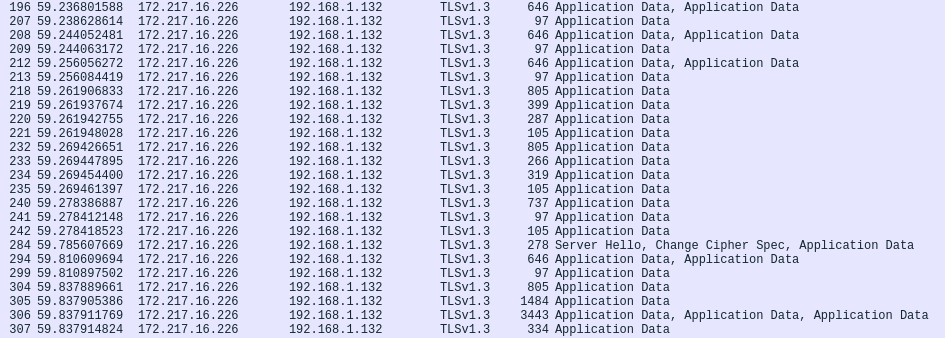
\includegraphics[scale=0.3]{img/paquetes-media.png}
	\end{figure}
\end{itemize}

Haciendo los cálculos, el tamaño medio de cada paquete enviado por \textit{spotify} es de 372.96 bytes. No obstante, cabe destacar que el tamaño entre paquete y paquete puede variar mucho, como se ve en la imagen siguiente, lo cual es un comportamiento algo sospechoso. No sería extraño suponer que \textit{spotify} envía paquetes pequeños con datos basura, que no supongan un coste alto de ancho de banda pero que puedan despistar a todos aquellos que estén captando paquetes en la red.

\begin{figure}[H]
	\centering
	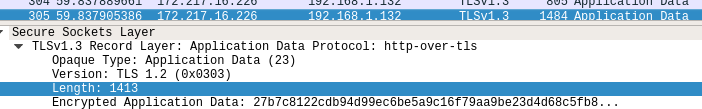
\includegraphics[scale=0.3]{img/paquete-grande.png}
	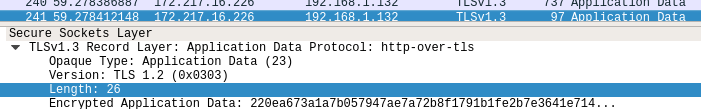
\includegraphics[scale=0.3]{img/paquete-smol.png}
\end{figure}

\subsection*{Datos relacionados con el envío de paquetes}

\begin{itemize}
	\item \textbf{Protocolo de transporte:} \textit{spotify} envía los paquetes a través de TCP. Aquellos que contienen datos (fragmentos de la canción) además van cifrados, por lo que usan TLS. Algo curioso es que en mitad del envío de paquetes, \textit{spotify} cambia el cifrado que está utilizando, lo que en ocasiones le lleva incluso a cambiar la versión de TLS. Además puede enviar más de un paquete de datos a la vez. Este hecho se puede observar en la siguiente imagen:
	
	\begin{figure}[H]
		\centering
		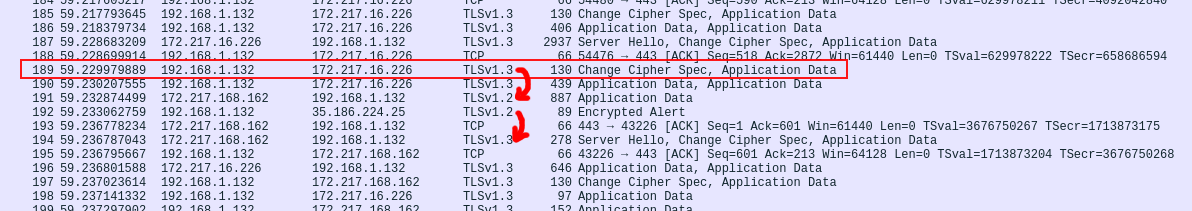
\includegraphics[scale=0.35]{img/patron-change-cipher.png}
	\end{figure}
	
	Es un patrón de envío que siguen durante el envío de paquetes para asegurarse de que, si hay alguien escuchando en la red y captando los paquetes, tenga que cambiar rápidamente de descifrador entre paquete y paquete, lo que evita, o al menos dificulta mucho, que los atacantes puedan descifrar el contenido enviado.
	
	\item \textbf{Puerto:} el puerto que recibe los paquetes es el 443. \textit{Spotify} utiliza \textit{port forwarding}, es decir, introduce la información dentro de paquetes con otro protocolo por encima; por ejemplo en este caso introduce los datos de la canción en un túnel \texttt{HTTPS} y los envía, y cuando llegan al dispositivo entran por el puerto de \texttt{HTTPS}. Si el puerto 443 está capado, también puede utilizar el 21 (\texttt{TCP}) o el 80 (\texttt{HTTP}).
	
	\item \textbf{Frecuencia de envío}: como es lógico pensar, la frecuencia de envío varía según las necesidades de datos del dispositivo y el tamaño de los paquetes enviados. Si los paquetes que se envían contienen muchos datos para reproducir una canción, la frecuencia será menor. También depende de la canción que se esté escuchando y del plan que tengamos en la aplicación (cuando es premium la música tiene mejor calidad, por lo que es normal pensar que la cantidad de datos es mayor).
	
	Ya que para calcularla solo necesitamos el tiempo de un paquete a otro y la columna de tiempo está presente (segunda columna en wireshark, medido en segundos), he utilizado los 1052 paquetes para sacar una media lo más cercana posible a la realidad. La diferencia entre el envío de paquetes de uno a otro es muy pequeña. Un fragmento de la diferencia de tiempo entre envíos es el que se ve en la siguiente imagen de excel:
	
	\begin{figure}[H]
		\centering
		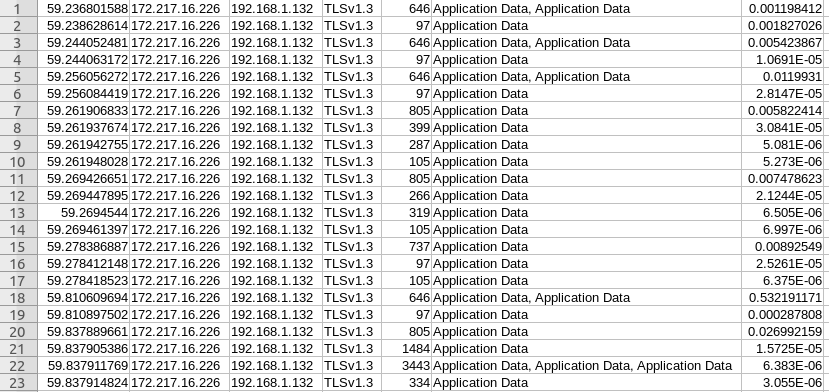
\includegraphics[scale=0.35]{img/fragmento-tiempos.png}
	\end{figure}
	
	Tras hacer los cálculos, la frecuencia media de envío de paquetes es 0.08381 segundos, es decir, cada 83.81 milisegundos más o menos se envía un paquete con datos de la canción para que se siga reproduciendo.
	
	\item \textbf{Bitrate medio}: para calcular la tasa de bytes media necesitamos dividir el número de bytes enviados de un paquete entre el tiempo que ha tardado y hacer la media entre todos. Utilizando el archivo \texttt{.csv} con los datos de la captura, calculamos la media. Salen aproximadamente 7 MB/s, la cual es una velocidad bastante buena.
	
	\item \textbf{Bitrate pico}: para calcular el pico debemos buscar el bitrate máximo entre la tasa de cada paquete individual. Al haber un número de paquetes tan grande, se podría decir que he conseguido capturar un paquete que ha sido enviado especialmente rápido ya que ha dado lugar a una tasa de 10.14 MB/s. Ese paquete se corresponde con el envío 219, como se puede ver en la imagen de la captura de wireshark (la tasa calculada se ve en la segunda imagen, en la última columna):
	
	\begin{figure}[H]
		\centering
		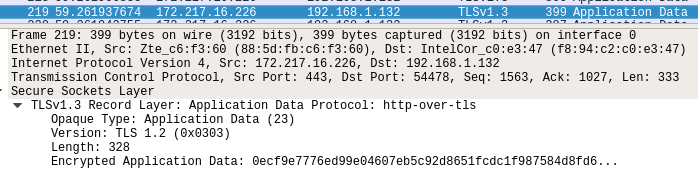
\includegraphics[scale=0.5]{img/pico-wireshark.png}
		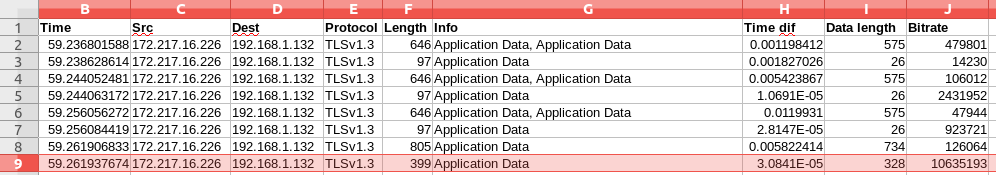
\includegraphics[scale=0.35]{img/pico-excel.png}
	\end{figure}
\end{itemize}

\end{document}